% 学习与科研.tex
% Auto-generated from 感悟论语.odt by tools/odt_to_tex.py

\setpartplant{artwork/bamboo.png}
  {绿竹 · 《诗·卫风·淇奥》}
  {如切如磋，如琢如磨。}
  {《论语·学而》}
  {学习与科研}
\part{学习与科研}

\chapter{PhD Manifesto（博士宣言）}

\begin{classic}
《论语·为政篇第二 2.12》子曰：「君子不器。」
\end{classic}

\begin{itemize}
\item A PhD should not be one of the inlays on the edifice of an organization.
\item A PhD should not be an underling of the capital system.
\item A PhD should not pompously claim combinatorial variations as innovation.
\item A PhD should not degenerate from a maker into a user.
\end{itemize}

\entrydate{2020.06.19}

\chapter{博士的使命与独立研究}

仅就我曾经做过相关研究的学科而言（包括电介质物理、电磁场数值计算、计算数学），每个领域都有对于从事该方向研究的学者来说根本绕不过去的来自西方的学术专著与专业软件。能够在完备性、准确性、细致性、严谨性、原创性等品质上与之相提并论的国产学术专著与基础软件仍旧很少，有些领域甚至是空白。这一点想必每位攻读过博士学位的同学都会深有体会。大体上讲，中国近现代科学研究的开展是根植于西方科学体系（包括理论与工具）之上的。如果我们不能甘心坐冷板凳将国外的这些成果承接过来，予以全面、系统地吸收、消化，也就不用提在此基础上能有什么原创性、本质性的创新成果了。

因此，作为生活在中国的中国人以及作为这个教育体系培养出的博士，不论我们当下是否身处学术圈内、体制内，面对这样的情况其实每个人都责无旁贷。我们需要有属于自己的基础数学算法库和科学仪器，不能只满足于利用非诞生于我们自己双手的现有仿真工具去做一些应用型工作或用昂贵的进口设备去测得一些实验数据。如此即便能够获得一些对国家“有用”的短期成果，能够让资本炒作、业界吹嘘，变为在任官员和领导的政绩，但对于学者自身而言，这样的做法会使我们始终受到工具能力的限制，且关键是缺乏接触底层理论、细节逻辑和精妙技艺的实践机会，从而浪费了上天赋予我们本该用以成为更好的自己、不断逼近人类最优秀科学家和匠人的巨大潜能。

一流的物理学家往往都是自己磨镜片、造仪器。我们也应以之为榜样，写出属于自己的算法代码，做出属于自己的科学仪器，把核心技术真正掌握在自己的手里。如果能有更多的人以这样的价值观不断夯实自己的理论和技术能力，开展科研和技术攻关以打通纯粹理论与工程实践之间的鸿沟，做成一批真正能够实用的基础算法库和仪器，那么良好的科研生态就能在国内逐渐形成、扎根。纯粹的理论研究与工程实际之间的距离或者逻辑链条可以很长，时间跨度也可以很大，但二者之间绝不能是割裂的。年复一年地发文章但始终见不到工程上的应用，这样的研究工作恐怕只对从事该研究小团体的私利有益，浪费的则是并不富裕的老百姓的血汗钱。中国的改革开放和大学科研与外国学术界的交流、接轨已四十余年。论智力我们自信且自豪地认为并不比外国人差。但如果这么多年都过去了我们还在一些重要的科技领域没有突破，仍被人卡着脖子，那也不要怪世界没有给我们时间和机会。

真正有品质的研究、缜密精巧的算法、设计精良的高性能软件单靠当前运作模式与评价体系下的学校或者科研院所其实是没有指望的。这就需要尤其是因为散落在体制外而相对容易做到思想自由、精神独立、行动与方向可控的诸多博士能够迎难而上，摒弃将科学与工程割裂开来的错误的“二分法”思维，通过做真正的研究、做实实在在的底层技术与基础软件，打磨与完善自己的理性与手艺，实现真正意义上的自我“救赎”，并由此创造出经济价值。如此先有了源自诸多个体的自我“救赎”，在当前的学术体制与评价体系之外塑造追求科学真理、崇尚工匠精神、培养科技审美的良好氛围，才能最终形成一股净化学术圈内诸多不正常现象的不尽源泉。如此充分发挥每个人的能动性，实现“克己复礼”，难道不正是科学的第一推动力么？

\begin{classic}
《论语·颜渊篇第十二 12.1》 颜渊问仁。子曰：「克己复礼为仁。一日克己复礼，天下归仁焉。为仁由己，而由人乎哉？」颜渊曰：「请问其目？」子曰：「非礼勿视，非礼勿听，非礼勿言，非礼勿动。」颜渊曰：「回虽不敏，请事斯语矣！」
\end{classic}

\entrydate{2020.09.28}

\chapter{打破工科研究的限制}

\begin{classic}
《论语·雍也篇第六 6.12》 冉求曰：“非不说子之道，力不足也。”子曰：“力不足者，中道而废。今女画。”
\end{classic}

工科中常见的研究模式是从实际应用出发，在现有的理论中寻找依据，再组合运用现有的或者发明新的技术，以解决具体问题。工科研究这种实用主义的“禀赋”从一开始便决定了其并非是追根溯源的。在这种模式的驱动下，虽然也能做事、出结果，但却无法获得真正意义上的——即纯粹理性的、彻底的理解，并最终反过来限制其自身的提升与发展。

虽然在工科研究中我们也会经常遇到数学公式，但其中的逻辑推理并不完整与彻底，每一个环节也经不起严格的推敲。若研究者在工科的范畴内寻根究底地问下去，最终得到的仍是疑问和悬而未决——对于这一点，若以数值仿真为例，只要我们对比一下工科与数学学科对有限元方法的阐述就可以明白。因此，我觉得工科研究大多仅是借用了数学的表达形式来获得一种本质上仍是定性的、维象的解释，并用以“自欺”。由“自欺”导致“不知道”、“不理解”，从而无法做出本源性、原创性的创新。这也便是为什么我们国家在高科技领域被西方卡脖子后才逐渐意识到发展基础学科的重要性。

对于工科领域的研究者而言，虽然其所从事的研究工作是从现实与实用性出发的，但其自身学习与探索的过程却是在理性的推动下一步步展开的——这是由人类的认知模式所决定的。除了理性的不够完整与彻底外，这个过程与理科领域的研究者并没有任何不同。所以，将自身归入工科阵营其实是一种急功近利、划地自限的实用主义二分法（dichotomy）。为了改变这个现状，以获得真正意义上的理解与自圆其说，工科领域的研究者虽然不必拥有提出新的基础理论的能力，但完全应该能够读懂和理解已有的基础理论成果。只有如此，才能将纯粹理性推及现实应用，使科学与工程有机结合，得到更多原创性的成果。

\entrydate{2021.03.07}

\chapter{顶天立地的研究}

研究生时期，我们系里的王赞基老师曾教导同学们要做“顶天立地”的研究。所谓“顶天”，是深入、扎实地学习与研究基础理论，达到高屋建瓴的境界。所谓“立地”，则是将基础理论通过工程技术方法准确、可靠、有效地实现出来，以解决现实问题。经过多年的学习与研究实践，我对这个原则也有了更多的体会，总结如下与大家分享交流。

\begin{itemize}
\item 顶天的意义
\end{itemize}

\begin{itemize}
\item[]
\begin{itemize}
\item 只有以基础理论作为支撑，我们才能将貌似不同的众多具体问题抽象为较少的几大类问题，然后再以通用的数学方法统一求解，从而降低了工程问题的复杂度，也避免了因重复求解类似问题带来的麻烦与可能的错误。
\item 要将全面、系统学习基础数学与物理理论作为重要但不紧迫的长期任务，一以贯之、不计利害、终其一生地坚持下去。虽然“吾生也有涯，而知也无涯”，但只有在这个解惑、求真的过程中，才能令我们坚韧不拔的精神得到充分的培养，使我们理性的光芒得以充分发挥和绽放。
\item 孔夫子通过“有教无类”以求实现人在精神、意志、人格上的平等。而我们恰恰能够在与名利无关的纯粹的基础理论学习中，“克己复礼”，践行夫子的伟大理想。\par 《论语·卫灵公篇第十五 15.39》 子曰：“有教无类。”\par 《论语·颜渊篇第十二 12.1》 颜渊问仁。子曰：“克己复礼，为仁。一日克己复礼，天下归仁焉。为仁由己，而由仁乎哉？”
\end{itemize}

\end{itemize}

\begin{itemize}
\item “顶天” → “立地”：因为知识是永远也学不完的，所以为了在“顶天”的同时“立地”，我们也要能够及时地从寻根究底的纯粹理性中跳出来，围绕需要解决的具体问题和待实现的软硬件功能，挑选出与之直接相关的理论成果，予以快速实现、验证、产品化。正如夫子所强调的知行合一：“多闻，择其善者而从之。多见而识之，知之次也。”。\par 《论语·述而篇第七 7.28》 子曰：“盖有不知而作之者，我无是也。多闻，择其善者而从之。多见而识之，知之次也。”
\item “立地” → “顶天”：在具体的开发过程中，每每遇到因理论知识不足而陷入不解与困顿的时候，工程上的“试错法”与“打补丁”已不再奏效——即便能暂时应付，也往往是极其糟糕与丑陋的实现与设计。此时，便要收起“急功近利”的心思，宁神专注，进入理论的海洋深度下潜。夫子说的“吾尝终日不食，终夜不寝，以思。无益，不如学也。”正好在这里适用。\par 《论语·卫灵公篇第十五 15.31》 子曰：“吾尝终日不食，终夜不寝，以思。无益，不如学也。”
\item “顶天”与“立地”两种模式均需要一丝不苟、点滴积累、不断迭代。面对看不懂、搞不通的困境，仍要坚持阅读专著、文献、代码、文档。只有持续的努力才能最终换来解开谜团的“好运气”。
\end{itemize}

\entrydate{2021.05.13}

\chapter{被封的谷歌与大师之路}

在国内做科研和技术相关工作的人想必对无法访问谷歌——尤其是谷歌学术搜索——一直耿耿于怀吧！我在做博士研究期间就屡次为此感到困扰。直到2010年谷歌退出中国后，这种不便才彻底成为难以改变的现实。当时的我甚至为此愤愤不平，仿佛科研的天空也都变得黯淡无光了。之后，因为尚未有哪个搜索工具能与谷歌及学术搜索匹敌，我搜索文献的效率、数量、质量均有所下降。尽管如此，日子也还是照常地过，科研亦未曾中断。再掂量一下自己的理论功力与科研水平，似乎也并未因谷歌的退出与存在而有所损益。自然地，这样的问题便浮现于我的脑海：谷歌给我们带来的信息究竟具有什么样的属性？能够对我们产生哪些帮助？除此之外，还有哪些能让我们成为出色的行业专家甚至是大师的必要条件？

我的观点是，从搜索引擎得来的信息基本上属于“常识”的范畴，即对于已存在“事实”的直接描述、表征。即便它们显得非常专业和抽象，甚至要借助复杂的数学符号才能表达，比如维基百科给出的学术相关的词条，那也只不过是相关专业领域中的常识。你觉得它们难以理解，是因为你所积累的用于理解它们的必要基础常识还不够多。其实，经过一段时间的熟悉，完全理解它们并不是问题——在这里，更高的智慧尚无用武之地。再举个例子，对于那些进入大学科研阶段之前的孩子，如果他们相较于同龄人显得见多识广，像是知天文、晓地理吧，家长往往会欣喜万分，即所谓在起跑线和马拉松赛跑的前五公里领了先。其实这个阶段的孩子所掌握的基本上是常识性的知识，是丝毫不值得骄傲的：因为对任何人来说，即便之前没有接触过这些知识，都可以借助网络搜索在很短的时间内理解。可以说，互联网发展至今，以其随处伸手可得的海量数据弥补了人们以往因为所处阶层与地域不同而在常识性知识资源占有量上的差异。比如，个人藏书，所在区域的书店和图书馆数量以及藏书量。

可如果想要成为行业专家与大师，常识掌握得再多也还是远远不够的。它们像是给身体虚弱空乏的人注入的葡萄糖，仅能够维持其基本生命，但根本无法解决更高层次的生理与心理需求。所以，在常识之外，技能、理论与思想是必不可缺的。下面分别予以说明。

所谓技能，就像是卖油翁所说的“惟手熟尔”，即俗称的手艺。它依靠的是在正确原则与训练方法指导下的大量反复练习，而无法直接从常识中产生，更不会产生新的常识。虽然，这个反复训练的过程只是验证了已有的常识，但却是由“认识到”演变至“能做到”的必经之路。比如，数学公式与逻辑分析的推演，炉火纯青的乐器演奏技艺，能将想法变为软件的编程技巧。古人所谓“纸上得来终觉浅，绝知此事要躬行”就是这个道理。可以看出，只有当自己的功力达到足够火候，乃至转变为条件反射、固化到自己的基因中时，才能算是掌握了一门技能。这其中所需的持久专注与大量心血绝非一般人能及。这也就是为什么我们在学术界会看到一些夸夸其谈但并无实料的专家，在公司则是想法多且新颖但却做不出产品的工程师。

理论则是借助抽象，尤其是基于数学方法的抽象，对纷繁芜杂的常识进行简化、分类、统一的产物。它对常识中似是而非的概念予以清晰和精确无误的定义、界定，用公理、定理在不同的概念之间建立起极其复杂且精密的逻辑与定量关系。也许，理论所欲表达的道理是简单而形象的，但其表述形式与推演过程往往是抽象与深奥的，其目的就是为了将看似不同的现象归类后在统一的层面上考量。举例来说，对于搞电路的，需要认识到是动力系统的观点在统领着力学与电学两个完全不同领域的现象；对于搞电磁场的，要明白麦克斯韦方程中的标量与矢量均为不依赖坐标系的反对称张量；对于搞数值计算的，要理解如何将有限差分和有限元方法放到同一个理论框架下去分析。由此，只有对系统性的理论框架乃至整个大厦有充分的理解与掌握，我们才会说这个研究者是有理论修养和科学品味的。

思想是指依赖智慧、灵感与深刻的洞见，提出新的理论，再用自己纯熟的技能加以实践，并由此产生诸多新的常识。这一点像是道家所说的“道生一，一生二，二生三，三生万物”。也只有像费曼、爱因斯坦那样的大师才能达到如此的境界！因为这个境界早已非即便是颇有天赋和用功的人能及，这里便不再多说了。

通过以上的分析，是想让大家更明白地看到位于常识之外的技能、理论与思想的重要性，从而在科研中苦练内功、大量训练的同时，更多地发挥自身主观能动性，为产生原创性思想提供更多的机会。对于这一点，我国固体物理学家黄昆先生的做法就很值得借鉴：

\begin{classic}
大多数具有学术上的开创性与重要性的研究都不是繁复的，我的学识和驾驭知识的能力都很有限，之所以能有一些成果，关键是少而精，有了学习和研究的主动性，站在前人的肩膀上而又不被前人束缚住。……我文献看得比较少，因为那样容易被人牵着鼻子走，变成书本的奴隶。自己创造的东西和接受别人的意见，对我来说，后者要困难得多。学别人的东西很难，而自己一旦抓住线索，知道怎么做，工作就会进展得很顺利。
\end{classic}

总之，学者不能满足于知识的简单获取与了解，而应将其内化为自身的技能，并从中提炼出具有普遍性与统一性的理论，最终升华至思想与智慧的境界。这一点其实完全符合孔子所谓的“君子上达”的精神。

\begin{classic}
《论语·宪问篇第十四 14.23》子曰：「君子上达，小人下达。」
\end{classic}

\entrydate{2016.12.29}

\chapter{终生学习}

\begin{classic}
《论语·为政篇第二 2.4》子曰：「吾十有五而志于学，三十而立，四十而不惑，五十而知天命，六十而耳顺，七十而从心所欲，不逾矩。」
\end{classic}

我认为对于一个研究者而言，无论是工科还是理科，秉持“终生学习”的基本精神，坚持将功夫投入到如下三个方面是极其重要而有意义的：

\begin{itemize}
\item 不断地将知识理论化、纯粹化，以至于达到可以让机器处理和表达的程度。这时，若再往深处挖掘，则除了假设与公理之外别无他物——这是机械的、逻辑的理解。
\item 形成用定性、形象、简明的语言来概括与把握复杂概念和理论的能力——这是智慧的理解。
\item 在不同的理论知识之间、理论与应用之间发掘并建立更多的联系。这样的关联愈多，我们对于事物的现象、本质和运作机理的把握便愈加深入——这是统一的理解。
\end{itemize}

以上围绕“旧知识”展开的工作相对于非原创性的所谓“创新”其实更为重要。因为它们乃是真正创新的根基与土壤。

终生学习所跨越的时间尺度远远大于一般的长期计划，因此需要以不同的思想和心态来面对。

\begin{itemize}
\item 坚定信念，不要因进展的缓慢、过程的漫长、终点（看似）的“遥不可及”而有任何动摇和怀疑。
\item 时时督促与自我提醒，保持初心与深度工作的状态，以防止在漫长的时间河流中逐渐地、不知不觉地松懈下来。
\item 虽然所学的理论知识与磨练的技能跟当下正在做的事情与项目没有直接关系，但依然要完全认可这种学习与练习的价值。即，学习本身即是根本目的、技术本身亦能升至艺术境界，而不在于因为知识与技术的运用而带来的现实利益。因此，需要每日坚持。
\item 认识到回顾与复习同样也是学习，甚至是学习新知的重要途径。在曾经求学、求职的道路上，我们往往只在意学习的推进速度（快），知识的堆砌量（多），以及浅层次运用带来的“立竿见影”的效果，并以为这便能突显一个人的能力与才智。然而，我们却忽略了本质的理解和对底层技术的掌握。因此，温故知新便极为重要，“退”亦是进。
\end{itemize}

\entrydate{2021.02.15}

\chapter{好之者不如乐之者}

\begin{classic}
《论语·雍也篇第六 6.20》 子曰：「知之者不如好之者，好之者不如乐之者。」
\end{classic}

孔子说：“知之者不如好之者，好之者不如乐之者”。倘若没有淡泊宁静之心以及追求至善之地的锲而不舍，想必也难以真正领会这句话的含义。毕竟大多时候，无论是对于传诵已久的名言警句与圣人语录，还是当下在微博、微信上广为传播的美文妙语，人们表示欣赏和赞许是件很容易的事。但能否在更深层次上将其领会，付诸实践，乃至固化为自己的习惯，则颇为困难。要做到这一点，往往需要一些机缘来提供特殊的现实经验与心路历程，从而产生与积习断绝的决心以及自我革新的持久激情。对于自己目前的学习而言，若能将发现问题、体验困难作为人生的一大乐趣，那么即便自己还没有什么成果产出，就已经可以将自身的境界再提升一个层次了。试想，若一个学者从未体会到求知过程中的异常艰辛，又怎能由知之、好之升华到乐之呢？因此，没有经历百般的折磨与苦痛，也便无法领略“乐”的真正滋味。昔者颜回乐处境界之高，也是基于同样的道理。

由以上体会产生的过程也可以看出，尽管文学与艺术并不像实际理工科的理论与技术那样实在、有用，不会直接产生价值与成果，但是在人生道路上的百转千回中，它们却是深刻感悟与透彻自省的源泉。它们提供的是如灯塔般引领人生方向的大智慧。它们亦像是在手中把玩的温润玉器，提供的是隽永的生活情趣。它们也像是来自上帝的声音，在人生最为孤苦无聊之时，赋予我们所从事的枯躁事务以特殊的意义。无论在我们的人生历程中面对什么样的人，做什么样的事情，总是需要智慧、情趣与意义的吧！而这就需要我们多读书，多欣赏不同形式的艺术，以拓宽自己的人生维度。

\entrydate{2016.05.28}

\chapter{数值计算中的工匠精神}

我之所以要提倡工匠精神，不是为了响应国家号召，也不是为了迎合市场需求，而仅仅是因为它完全符合论语所倡导的“如切如磋、如琢如磨”、“君子上达”、止于至善的纯粹而普适的原则。而且，鉴于工匠精神和与之相称的技艺培养之难，一个优秀的科学工作者应当终生秉持这种亲力亲为、兢兢业业的精神才有可能臻于理想的境界，而不是在小有所成乃至功成名就之后便升格（堕落）为科研工作的组织者和资源的调动者。

仅就数值计算研究领域来说，工匠精神应当包括如下三个方面。

\begin{itemize}
\item 构建起完备的基础理论体系。可以随时随地如数家珍般地讲解、推演其中的任何一部分内容。这就如同演奏家（virtuoso）能够流畅娴熟地表演他们的保留曲目。
\item 具备通过亲自编程将理论方法付诸实践并塑造出精品软件的设计思想与高超手艺。与之相比，只能做出用作教学或演示的代码则是远远不够的。这是因为，能够真正实用的算法在理论基础、设计思想与开发方法上均与简单的演示程序有本质上的不同，需要长期的专门学习与训练才可掌握。
\item 修辞立其诚。能够通过写作、报告、讲座等形式，精确、形象、深入浅出地阐释算法原理，起到传播思想与知识的效果。这也是“己欲立而立人，己欲达而达人”的具体体现。
\end{itemize}

\begin{classic}
《论语·学而篇第一 1.15》 子贡曰：「贫而无谄，富而无骄，何如？」子曰：「可也，未若贫而乐，富而好礼者也。」子贡曰：「诗云：『如切如磋，如琢如磨』，其斯之谓与？」子曰：「赐也，始可与言诗已矣，告诸往而知来者。」

《论语·宪问篇第十四 14.23》 子曰：「君子上达，小人下达。」

《论语·雍也篇第六 6.30》 子贡曰：「如有博施于民，而能济众，何如？可谓仁乎？」子曰：「何事于仁，必也圣乎！尧舜其犹病诸！夫仁者，己欲立而立人，己欲达而达人。能近取譬，可谓仁之方也已。」

《乾卦·文言》 子曰：君子进德修业。忠信所以进德也；修辞立其诚，所以居业也。
\end{classic}

\entrydate{2020.11.20}

\chapter{坚持学习数学的价值}

有如长时间跑步或游泳总会有一个不适期，而坚持过了那个阶段后便不再感到疲惫一样，我现在的数学学习也正处在最为难受，随时都可能放弃的时候。而这也恰恰是最需要坚持的关键时刻。试想，如果有这么一种坚持，它能够使人舒舒服服地养成好习惯，轻轻松松将困难的任务达成，或者如上帝眷顾般地实现梦寐以求的理想，那它也就算不上是坚持了，或者说已被大打折扣。当我们觉出肉体上的苦痛、精神上的折磨，发现仍然行动不辍，即便是步履缓慢却也未曾放弃，这种状态正是我们应该予以认可与欣然接受的！

还有一个困挠我的问题是，正在学习的数学理论与工作项目所需的技术没有任何直接与短期的关系。即便从长远来看，二者之间何时能够产生联系并达到相得益彰的效果似乎也是遥不可期。如果我的学习效率不能提高，研究没有显著的进展，且总是如井中蜗牛般地前进五步、后退四步，那么目前的学习于己于人究竟有何实质的价值与意义就无法说清了。对于逐步走向平庸与无能的自我，那个已无改变世界甚至自我的勇气而只能无耐接受现实的自我，恐怕只能从数学学习中得到些许心理安慰与精神寄托吧！

可一切果真如此么？仔细想来，似乎仍有那么一线希望。数学学习与阅读名著小说不同，它绝不是打发与消磨时间的工具，也不是为了自娱自乐或提高个人修养——除了文明礼貌、举止行为优雅外，个人修养的提高所能带来的价值是极为有限的。其关键在于纯粹理性与锲而不舍的探索精神对自己人生的支撑，以及由此可能产生的对人类智慧宝库的贡献。可以说，这种活动本身便是对自我精神与意志自由的最好证明。它所遵循的原则是以真理为准绳，而无需为任何情面作出妥协与伪装。它不会使你自己成为别人的提线木偶，或者因精神空虚而只剩下如昆虫尸体般遇风即碎的躯壳。

既然数学学习尚存这么一线希望，那么就需要把它作为终极目标确定下来。子曰：“吾十有五而志于学，三十而立，四十而不惑”。与圣人相比，我们所拥有的后天物质条件要更加丰盈，接受教育的机会更多，质量也更好。然而，曾经的我堕落到连自己都觉得俗不可耐的地步，最根本的原因就是没有立志，没有一个终极目标。没有志，则不会一以贯之地去学。即便年至三十，在物质上算是立住了，但在个人的学识与思维水平上还远远未及而立的程度。待到四十，恐怕也根本谈不上什么不惑。需要明白，这个不惑，并非对社会上的规则与潜规则，以及左右逢源所需的伎俩而熟稔，而是对自我人生追求与理想的明确以及由此产生的始志不渝。

\begin{classic}
《论语·为政篇第二 2.4》 子曰：「吾十有五而志于学，三十而立，四十而不惑，五十而知天命，六十而耳顺，七十而从心所欲，不逾矩。」
\end{classic}

\entrydate{2016.09.22}

\chapter{教师节随想}

“师者，所以传道、授业、解惑也。”现在想来，给我深刻启迪、感动和慰藉，从而形成生命助推力的要属高中老师。在远离一二线城市，教学与信息资源都不丰富的地方，他们毫无保留地将自己掌握的知识、形象且深刻的体会传授给一届届的学生，真诚与无私地向他们阐释什么是正义与纯粹，什么才是人生中的至真至善。他们不但如严父慈母般地关心学生的生活细节，还像是伯乐一样发掘与培养他们的优点与潜力，使其认识到自己的出色和与众不同——我至今能够用类似牛顿那个时代的科学家进行研究和探索的方式，即建立在理性基础上的形象阐释与哲学思考，去学习数学、物理，便是高中物理老师的恩赐。而当一个人进入大学乃至走向冷漠与功利的社会，这些生命的助推力便像是免费的午餐不再可能。春蚕到死丝方尽，蜡炬成灰泪始干！高中老师们就像是科幻作家刘慈欣笔下的那位乡村教师，看似渺小卑微，但对人一生的教化与引导，突显了人类存在的价值与意义，其影响波及整个宇宙！

由此，进一步阐发一直以来想表达的观点：纯粹的知识，永恒的真理，艺术的至善之美，以及它们所带来的感动与震撼，对于每个人来说没有地域、阶层、职业、贵贱的限制，是最最公平的。只要愿意，即便在信息与资源匮乏的年代，你仍旧可以与科学的真知对话，艺术的大门也始终向你敞开！即便身居陋巷、箪食瓢饮，也完全可以做到学识的丰富与修养的深厚。孔子所说的有教无类也便包含这个意思。

\begin{classic}
《论语·卫灵公篇第十五 15.39》 子曰：「有教无类。」

《论语·雍也篇第六 6.11》 子曰：「贤哉，回也！一箪食，一瓢饮，在陋巷，人不堪其忧，回也不改其乐。贤哉，回也！」
\end{classic}

\entrydate{2016.09.10}

\chapter{美丽心灵}

电影《美丽心灵》中的约翰·纳什缘何算得上是心灵美，以前我对此并不理解。一位荣获诺贝尔经济学奖的大师，数学方面卓越的才华与能力毋庸置疑。但他只是沉浸于属于他的数学天地之中，还因自身的精神疾病给亲友、同事带来不少麻烦与痛苦，从中看不出丝毫中国人一般观念所认为的道德意义上的心灵美，更是毫无“感动中国”里提倡的那种自我牺牲与奉献精神。

如今，我终于理解了纳什的心灵之美在于他始终追求真理，在科研上保持了一贯的原则与风格，对事而不对人。这是一种纯粹之美，与儒家“君子固穷”的精神异曲同工。这种美也让我意识到，人生除了因为消极、被动地忙碌、吃苦而被褒奖，还有发掘、发现、发挥自我的更加积极的意义！而这同样与儒家“仁”的核心精神“克己复礼”相契合。

\begin{classic}
《论语·卫灵公篇第十五 15.2》 在陈绝粮。从者病，莫能兴。子路愠见曰：「君子亦有穷乎？」子曰：「君子固穷，小人穷斯滥矣。」

《论语·颜渊篇第十二 12.1》 颜渊问仁。子曰：「克己复礼，为仁。一日克己复礼，天下归仁焉。为仁由己，而由仁乎哉？」颜渊曰：「请问其目？」子曰：「非礼勿视，非礼勿听，非礼勿言，非礼勿动。」颜渊曰：「回虽不敏，请事斯语矣！」
\end{classic}

\entrydate{2023.02.18}

\chapter{算法开发与自我提升}

\begin{classic}
《论语·公冶长篇第五 5.14》 子路有闻，未之能行，唯恐有闻。

《论语·学而篇第一 1.15》 子贡曰：「贫而无谄，富而无骄，何如？」子曰：「可也，未若贫而乐，富而好礼者也。」子贡曰：「诗云：『如切如磋，如琢如磨』，其斯之谓与？」子曰：「赐也，始可与言诗已矣，告诸往而知来者。」
\end{classic}

围绕一个大系统而展开算法开发工作时，我习惯于每次只往框架内添加一个很小的功能——虽然小，但与之相配的文档注释却不能有所缺失；为了保证理论实现的准确性与实际运行的可靠性，还需要编写相应的单元测试。

与之类似，在自我修炼与自我提升的道路上，靠的也是点滴积累：每次只专注实践某一点，任务完成后加以总结、体会，形成内心的映照，再固化为自然而然的习惯。这便是子路”未之能行，唯恐有闻”的道理。

由此看来，面对无论是外在还是内在的\textbf{复杂系统 }，改进提升的基本方法都是类似的，均是践行”如切如磋，如琢如磨”的最好体现。

\entrydate{2021.07.16}

\chapter{吾将上下而求索}

我从学校毕业后就一直在外企的中国研究中心工作，并在很长一段时间里也都抱着做深入研究工作的幻想。然而，外企在其中国研究中心设立的项目与其本国研究中心项目的性质是截然不同的。仅就我个人的研究领域而言，在外企总部的研究中心，能够看到理论与工程的完美结合，而且这样的结合在中国最顶尖的高校与研究机构都是没有的。而在外企中国研究中心则根本无法触及核心技术，更不用说在相关的理论与技术方向上能够开展什么系统和深入的工作了。“名不正，则言不顺；言不顺，则事不成。”想要在外企中国研究中心从事真正的研究已然不可能。

这七年以来，我个人的状态可以说是在南辕北辙中积蓄知识、技术、能力、耐心。有这样坚持的精神固然是好的，但若在错误的方向上走得太久，即便待有了一定积累后重回正确的方向，也不见得再有充足的机会和时间让自己走得很远。

朱光潜先生在《谈修养》一书中讲到，“普通欧美人士说：‘生命从四十岁开始。’他们到了五六十岁时，还是血气方刚，还有二三十年可以在学问事业方面努力。”而我目前也正处在精力与智力充足的宝贵时期，而且几乎是在人生中能够有所作为、有所改变和有希望取得突破的最后一个时期。试想，再往后拖延五年、十年，那时的我虽然仍未退休，但是精力、智力、记忆力、视力恐怕都要衰退不少。届时若再想于理论和技术上有所突破、做自己想做和应该做的方向，将会为时已晚。

一天中最宝贵的时光就是白天的8个小时。而若像大多数人一样将这8个小时全部放在公司工作上，则下班回家后固然可以做一些属于自己的事情，但是人的精力、专注度、做事的效率和质量都已无法和白天的状况相比。如此长期积累，至多也就能养成个搏人眼球的“业余爱好”而绝非“专业”。“巧妇难为无米之炊”，在时间资源严重不足的情况下谈时间管理是没有意义的。

随着年龄的增长，一个人的时间理应变得越来越贵。因此，反而应该让自己的思路跳出金钱、名利的桎梏，更多地考虑该如何充分发挥自身的能力和无限的潜力，由此做一些于国家、社会正确有益的事情，创造更多的价值。

如果我不去尝试自己认为在理论的深度、技术的先进和设计的品味上正确的事业，则会留下终生的遗憾，而我也将成为彻头彻尾的懦夫和空想家！《论语·公冶长篇第五 5.20》 季文子三思而后行。子闻之，曰：「再斯可矣。」当一个人有了自己充分的理性思考，就应当做出决定并且坚决、果断地行动。

\entrydate{2020.08.21}

\chapter{贫而乐，富而好礼}

\begin{classic}
《论语·学而篇第一 1.15》 子贡曰：“贫而无谄，富而无骄，何如？”子曰：“可也，未若贫而乐，富而好礼者也。”子贡曰：“诗云：『如切如磋，如琢如磨』，其斯之谓与？”子曰：“赐也，始可与言诗已矣，告诸往而知来者。”
\end{classic}

若以科研类比此句“贫而乐，富而好礼”，便意味着学者在未占有充足科研资源的时候，当不离不弃地专注于学问本身，索隐探微、从吾所好、以之为乐，绝不会以“生存”为藉口而降低理性的要求与科研的\textbf{品味}、\textbf{质量}。在行动上，这就要求我们努力将资源型科研转变为智力型科研，将技术型科研转变为纯理论科研。这样看来，“坏事”反倒变成了好事：我们有了更多的机会用脑思考、用心体会，从而获得深入的理解，与真理的距离更近。

当学者拥有了一定学术地位时，则不应整日思忖着如何基于有利条件去争取更多的项目与资源，以便巩固已经到手的所谓“学术地位”；而是要让学术地位和资源为我们实现从应用层到理论层的提升服务，为回归至我们曾经渴求真知的初心服务，通过充分发挥理性的作用，向更为\textbf{纯粹}与\textbf{普遍}的学问发起挑战。这也正是庄子《让王》篇描述孔子与弟子们“在陈绝粮”而提到的“穷亦乐，通亦乐，所乐非穷通也。道德于此，则穷通为寒暑风雨之序矣”。

\entrydate{2021.10.01}

\chapter{闻过则喜}

大团队中项目管理的目的是有效控制乃至将风险降到最低。以这种方式向已有的平台与体系添砖加瓦毫无问题，但却根本无法用于基础与开创性的工作。对于后者，我们应反其道而行之，鼓励冒险：在保证数学与物理理论准确无误的前提下，开发过程中遇到的难题越多、风险越高——这是因为为了保证算法同时具有足够的抽象能力与生产力性能，往往需要用到更高级的思维与编程方式；为了实现工业级的质量而非教学演示目的，需要采用更先进的软件技术与开发方法——则意味着这项工作具有更高的不可替性，最终成果具有更强的统一性和更广的适用性。

以前，当我面临难题与风险时，容易出现失望、悲观、迷茫的情绪。当意识到了上述道理后，虽然迷茫仍在，但失望与悲观已被喜悦所取代：因为我坚信一个个问题终能被解决，它们逐步积累由量变产生质变，才是通向更高标准的成功、让学问更加笃实的唯一道路。这一点正好与子路的“闻过则喜”有异曲同工之处。

\begin{classic}
《孟子·公孙丑章句上》孟子曰：“子路，人告之以有过，则喜。禹闻善言，则拜。”
\end{classic}

\entrydate{2021.10.07}

\chapter{君子上达}

\begin{classic}
《论语·宪问篇第十四 14.23》 子曰：「君子上达，小人下达。」
\end{classic}

昨日完成了ACA+ (Adaptive Cross Approximation)算法流程的\\ C++实现。虽然我对C++的高级用法和标准库已有一定了解，但在具体函数功能的调用与灵活使用上仍不熟悉。因此，整个开发过程实际上是伴随着编写C++测试代码缓慢而稳步地向前推进的。这样的做法虽然效率不高，但却在很大概率上保证了已完成代码的正确性、可靠性——而这对于将程序逻辑与数学理论深度揉合在一起的数学类软件来说是至关重要的。若没有细节上的把控，最终在程序调试的时候势必会产生“处处都可能是错误的来源，但又无法予以落实确定”的这种无助、无措的感觉。

再回顾我已往写过的代码，觉得一切既熟悉又陌生，甚至有些难以至信。曾经我以为遥不可及、高不可攀、只能忘洋兴叹的算法流程竟然都逐一地被理解与编码实现出来。这其中的滋味如同在黑暗中摸索前进，又仿佛在迷雾笼罩的汪洋大海上航行。往往是在经过了无数的迷茫、犹疑、动摇、痛苦之后，才终有微薄的收获。而且还必须始终与遗忘和生疏对抗，防止已经建立起来的知识、理解、技能随着时光的荏苒而付诸东流。

想来每个人的天赋与潜质都已由基因和命运所确定了的。就像是一颗参天大树的种子绝不可能长出杂草或灌木。然而，仅有这些先天的能力又是远远不够的，必须通过我们个人的不懈努力去发现、证明、发挥、提升自我，不断逼近天赋与潜质为我们设定的极限。因此，勇于不断地尝试那些令我们感到没有把握、易于迷茫无措的高风险工作，在这个过程中磨炼自己的意志、性情、手艺，应该是充分体现一个人价值与尊严的最好方式吧！

\entrydate{2022.03.11}

\chapter{君子不忧不惧}

应不断磨炼与优化我们做事时的情绪、心态。要做到有条不紊、处之泰然，正所谓“君子不忧不惧”。只有如此，才能让我们的科研生命愈加长久。

凡事都有其内在的节奏与规律。功夫不到、时机不成熟，却仍幻想与渴求成功的硕果实属庸人自扰。只要我们为志向全力以赴了，那么面对在一时得失以及某段人生的发展方面落后于他人的情况，就完全不必急躁乃至乱了阵脚。如同园中的繁花，每个人都是独一无二的品种，都有属于他自己热闹绽放的时节。人们不会因为秋菊与蜡梅的花期晚于早在春季便争芳吐艳的桃李而去对其加以责怪。相反地，反倒会因为它们为肃杀、萧索的秋冬点缀增色而感到由衷的喜悦和陶醉。对于草木尚能如此，看待人岂不更应秉持同样明智、豁达的态度？

\begin{classic}
《论语·颜渊篇第十二 12.4》 司马牛问君子。子曰：“君子不忧不惧。”曰：“不忧不惧，斯谓之君子矣乎？”子曰：“内省不疚，夫何忧何惧？”
\end{classic}

\entrydate{2020.12.11}

\chapter{学而时习，不怕重复}

数学学习的过程中往往遇到所学内容似曾相识，甚至是大量重复的情况。此时若是心气浮躁、失去耐性，追求进度，便会草率地跳至后续章节阅读。但是，由于书中推导涉及的条件以及用到的符号与以往所学仍有细微差异，而且这些差异虽小，但随着章节推进过程中的累积，到后面便会产生大相径庭的结果。由此导致跳到后续章节的学习难以做到扎实、稳妥，在数学严谨性的要求下必会“溃于蚁穴”，最终不得不翻回头来从头学起。这正所谓浮沙筑台，难以致远。

一般说来，看纯数学书和工科类应用型的书是大不一样的。前者重在明理，在于构建严谨自洽的逻辑细节与理论体系，若仅浏览其结论而无视推导过程及严谨性的话，就难有真正的收获，对其结论的理解也只是局部和片面的，甚至是错误的。而后者仅需做到“似是而非”的大体正确，能够即便是本质上错误或者维象地“解决”实际问题就好，对于真正的原理和逻辑推导是不予追究的。与此同时，研读纯数学书和文科类的书（如历史、心理、小说等）更是大大不同。后者往往仅需了解大意和把握主旨便能有所收获，而前者就不能如此“走马观花”般地随便了。

鉴于此，可以得出结论：数学学习不怕重复，且恰恰是贵在学而时习（习，既指复习，又指练习实践）、温故知新。绝不能因为急功近利、追求立竿见影的效果而失去系统化学习的耐心。

\begin{classic}
《论语 学而 1.1》子曰：“学而时习之，不亦说乎？”

《论语 为政 2.11》子曰：“温故而知新之，可以为师矣。”
\end{classic}

\entrydate{2017.10.06}

\chapter{见贤思齐，学无止境}

阅读文献与专著会时常遇到欲求甚解而不得的情况。即便是对于曾经学过的内容，若要重新以理性和严谨的数学方式寻根究底、“扪心自问”，反倒会愈加觉得自己的无知。面对大师的著作，“仰之弥高，钻之弥坚。瞻之在前，忽焉在后。……欲罢不能”。一时间，心生无尽的沮丧与失败感，简直是再正常不过了。可是，若依据篇首的引用理性地想一想，则所有悲观与颓唐的情绪实在是不必要的。相反，迎难而上、愈战愈勇才是正确的做法。更何况，无论是多么艰深的知识，虽然眼下看不懂，却不代表永远不能看懂。真正的人是动态发展和不断提升的。只要始终保持勤奋学习、踏实实践、点滴积累的作风，见贤思齐乃至最终赶超大师的水平便不是不可能。这样一来，与大师相比虽然晚些时候才到达科学之颠，但领略到的瑰丽风景是一样的。而且不仅如此，自强不息的求索与心路历程正是对儒家“止于至善”精神的最好实践，是人生不可多得的宝贵财富。

\begin{classic}
《论语·里仁 4.17》子曰：“见贤思齐焉，见不贤而内自省也”。

《论语·子罕篇第九 9.11》 颜渊喟然叹曰：「仰之弥高，钻之弥坚，瞻之在前，忽焉在后！夫子循循然善诱人，博我以文，约我以礼。欲罢不能，既竭吾才，如有所立，卓尔。虽欲从之，末由也已！」
\end{classic}

\entrydate{2017.09.27}

\chapter{见贤思齐的具体案例}

\begin{classic}
《论语·里仁 4.17》子曰：“见贤思齐焉，见不贤而内自省也”。
\end{classic}

今日清晨浏览多尺度仿真相关文献。看到了Martin Oliver Steinhauser所编写的专著“Computational Multiscale Modeling of Fluids and Solids”。其中的内容涉及数学、物理、软件设计与编程方法，体现出理论基础深厚扎实、内容详尽、研究范围广的特点。尤其是数学部分，从最基础的集合论讲起，再到拓扑学、微分几何、泛函分析、偏微分方程，给人很深的印象。

Martin Oliver Steinhauser是Fraunhofer公司的仿真研究专家与项目经理，曾领导了在德国全国范围内多家机构参与的多尺度仿真软件MMM-Tools开发项目，在10年的时间里拥有多达50万行代码的编写与开发经验。这充分表明他在融汇贯通从底层到面向应用的理论知识的同时，始终孜孜不倦地将其付诸实践。From theory to praxis，Martin的治学风格很好地体现了什么才是真正的博学、笃行，是值得我学习与追赶的榜样。同时，该书也启发我应当像海绵一样充分、快速地全方位吸收理论知识，以开放的心态与无畏的勇气勤勉研究，不给自己的记忆力、脑力、能力设置上限，永不满足。

最后，摘录出Martin给从事仿真工作的“用户”提出的建议：

\begin{classic}
I hope to convince those readers who consider themselves just users of ready-made software packages that it is very interesting to understand some of the common physical and mathematical principles on which these programs are based and, yet more important, that a thorough understanding of the functioning of a simulation code may enhance considerably the efficiency with which such programs are used.
\end{classic}

\entrydate{2022.08.20}

\chapter{学习莫要见异思迁}

今年三月开始在“喜玛拉雅”上听邓晓芒老师的《康德哲学》。采用一边听，一边记笔记，并将每章整理成思维导图的学习方式。本来是要一鼓作气学完的，但到了四月中旬，自己又半路开始看《南渡北归》三部曲。等这三大本看完，发现由于《康德哲学》学习起来更为枯燥、晦涩，且因为没有定期复习，所以再重新拾起来有较大的难度，于是就难以回到之前的节奏，转而开始读《A Mind for Numbers》了。对于数学理论的学习更是如此，因为其相对于哲学更加复杂，包含了千头万绪的细节，极为消耗智力，所以更难以重新拾起来，通过复习恢复至当初学习时的状态也要花很多的时间与精力。

由此可以看出，学习不要喜新厌旧、见异思迁，尤其是当看到了更加有趣也有益的理论、知识，最好仍先将手头的学习任务扎扎实实完成，甚至能够真正见到成效，之后再去尝试新的内容。这也就是《论语》中描述子路的那样：

\begin{classic}
《论语·公冶长篇第五 5.14》子路有闻，未之能行，唯恐有闻。
\end{classic}

再者，应当学而时习，不能中断。稍有中断，就容易丢掉辛辛苦苦累积出的良好状态。这时往往需要更多乃至数倍的时间与精力来复习、弥补，甚至是前功尽弃。

\begin{classic}
《论语·学而篇第一 1.1》子曰：「学而时习之，不亦说乎？有朋自远方来，不亦乐乎？人不知而不愠，不亦君子乎？」
\end{classic}

最后，还是要严格按照计划学习、复习、练习，从而不易受外界无论是有益还是有害信息的诱惑与干扰。

\entrydate{2018.08.03}

\chapter{悲观失望即是变相的浮躁}

虽然“学而时习”被安排在了《论语》第一篇的第一章，但是我与真正践行这句话的标准还相去甚远。一个常见的情况是，无论我在初学时将笔记记得多么认真、工整，时间一长且没有系统的复习和运用，便会将众多知识点及其相互联系都忘个一干二净。每每遇到此种情形，陷入无比的痛苦简直是再自然不过了：在那些悲观失望的时光中，书看不进去，什么事都不想做。待稍稍恢复后，却依然要直面先前遇到的尚未解决的难题以作出抉择：要么“只求大意”、“不求甚解”，则会埋下无尽的隐患与漏洞，最终只能落得浮沙难以筑台的命运。要么继续追本溯源，使在黑暗与未知中的“地牢”探索再下降一层。而回首来路，则又不知什么时候能够再回地面、重见天日。

我已经历了不只一回这样的局面，所以这次便能很快地重整旗鼓。清晨醒来，前一天晚上的困顿与颓唐业已消散。对于自己的初心、学习和研究应达到的标准、止于至善的终极目标也愈加确信和认可，以至坚不可摧。难道本来不正应该如此么：犹如在君子与小人之间做选择，要么择善固执，要么自行堕落，而从来就没有什么中间态，做真正的学问就是达到毫无错误、缺陷、疏漏、模糊的状态，以最终成就完美的境界。想要做出任何有创意、有突破的研究工作，想要打造任何精雕细琢的精品，也正是需要那种不计较任何利益、只是为了美之纯粹而一丝不苟、持久强行的精神。如果在这种状态与境界上有所程度的缺失或方向的偏离，则无论做多少“出彩”的工作、结多少丰硕的“果实”，都不过是南辕北辙，而且做得愈多，错得越多，自欺也愈多，只会与真理悖离得愈远。

有了以上的理解，如果面对种种困难、面对深不见底的知识海洋，在没有经过有计划、系统、持久的付出而产生的任何悲观与失望其本质都是过于浮躁、急于求成的表现。因为求胜心切，一个人才会变得没有耐心与毅力，也很难怀着一颗初学时的谦卑与放空的心态来投入足够的时间去重新面对、温故、知新。

\begin{classic}
《论语·学而篇第一 1.1》 子曰：「学而时习之，不亦说乎？有朋自远方来，不亦乐乎？人不知而不愠，不亦君子乎？」

《论语·为政篇第二 2.11》 子曰：「温故而知新，可以为师矣。」
\end{classic}

\entrydate{2019.06.19}

\chapter{思而不学则殆与问题树}

孔子说“思而不学则殆”，而我们在阅读学术文章的过程中，就往往会陷入百思不得其解的痛苦境地。此时，若继续冥思苦想，甚至开始怀疑自己的能力与智慧，消磨自信心，则是效率极低且难以达成目标的。这是由于我们目前已有的知识积累还远远不足以理解文章的内容和所蕴含的深刻思想。所以，若再像唐吉诃德般地苦读下去，收效不会很大。正确地做法是：按图索骥，阅读文章引用的文献，并根据疑难点重新整理关键词，再去搜索一批相关的文献、书籍、网文来阅读。只有这样在补充了一定的给养后，重新翻回头来再去读一开始受阻的文章，才可能会柳暗花明又一村，也才能真正有所收获。

由此也可以看出，这种研究方式就像是数据结构课学过的用于走迷宫的递归方法：每当看到一个单靠苦思冥想已经无法搞明白的问题，就要立刻将其压入堆栈。然后，从该问题引出若干新的分枝，并依次搜索每个分枝。如果在某些个分枝上又出现了新的问题，则又当将这些问题压入堆栈，并展开更深一层的分枝。当把某一层的分枝和子分枝问题都搞清楚后，再从堆栈中弹出一个问题并回溯到该问题。这时，因为大脑已获得了足够的信息输入，亦经过了多次的推导训练，这个在堆栈中可能保存了很久的老问题最终可以得到圆满的解答。

基于上述想法，我们可以对自己专注研究的一个或多个科研方向分别建立问题树，从而对我们在科学迷宫中所走过的路径以及要解决的问题进行有效地追踪。同时，也可以对不同层次的问题是否与实际问题的解决直接相关而加以澄清、划分——即，某些问题具有纯学术性质，是用来加深理解、提高理论修养、完善理论体系的，它们属于重要但不紧急的任务；而有些则属于可以解决实际问题的有效技术，它们决定了实际科研项目的进度，属于重要且紧急的任务。问题的树状结构意味着我们可以利用思维导图方便地将其组织与管理起来。只有如此，我们才不至于在科学的迷宫中走失，也不至于一辈子陷于纯理论学习而没有任何作为和实质性的贡献。

\begin{classic}
《论语·为政篇第二 2.15》 子曰：「学而不思则罔，思而不学则殆。」
\end{classic}

\entrydate{2016.12.03}

\chapter{Metaphor from Tiny Wings}

Tiny Wings is a lovely game on iOS. Its short introduction is written like this:

\begin{classic}
You have always dreamed of flying - but your wings are tiny. Luckily the world is full of beautiful hills. Use the hills as jumps - slide down, flap your wings and fly! At least for a moment - until this annoying gravity brings you back down to earth. But the next hill is waiting for you already. Watch out for the night and fly as fast as you can. Otherwise flying will only be a dream once again.
\end{classic}

\begin{center}
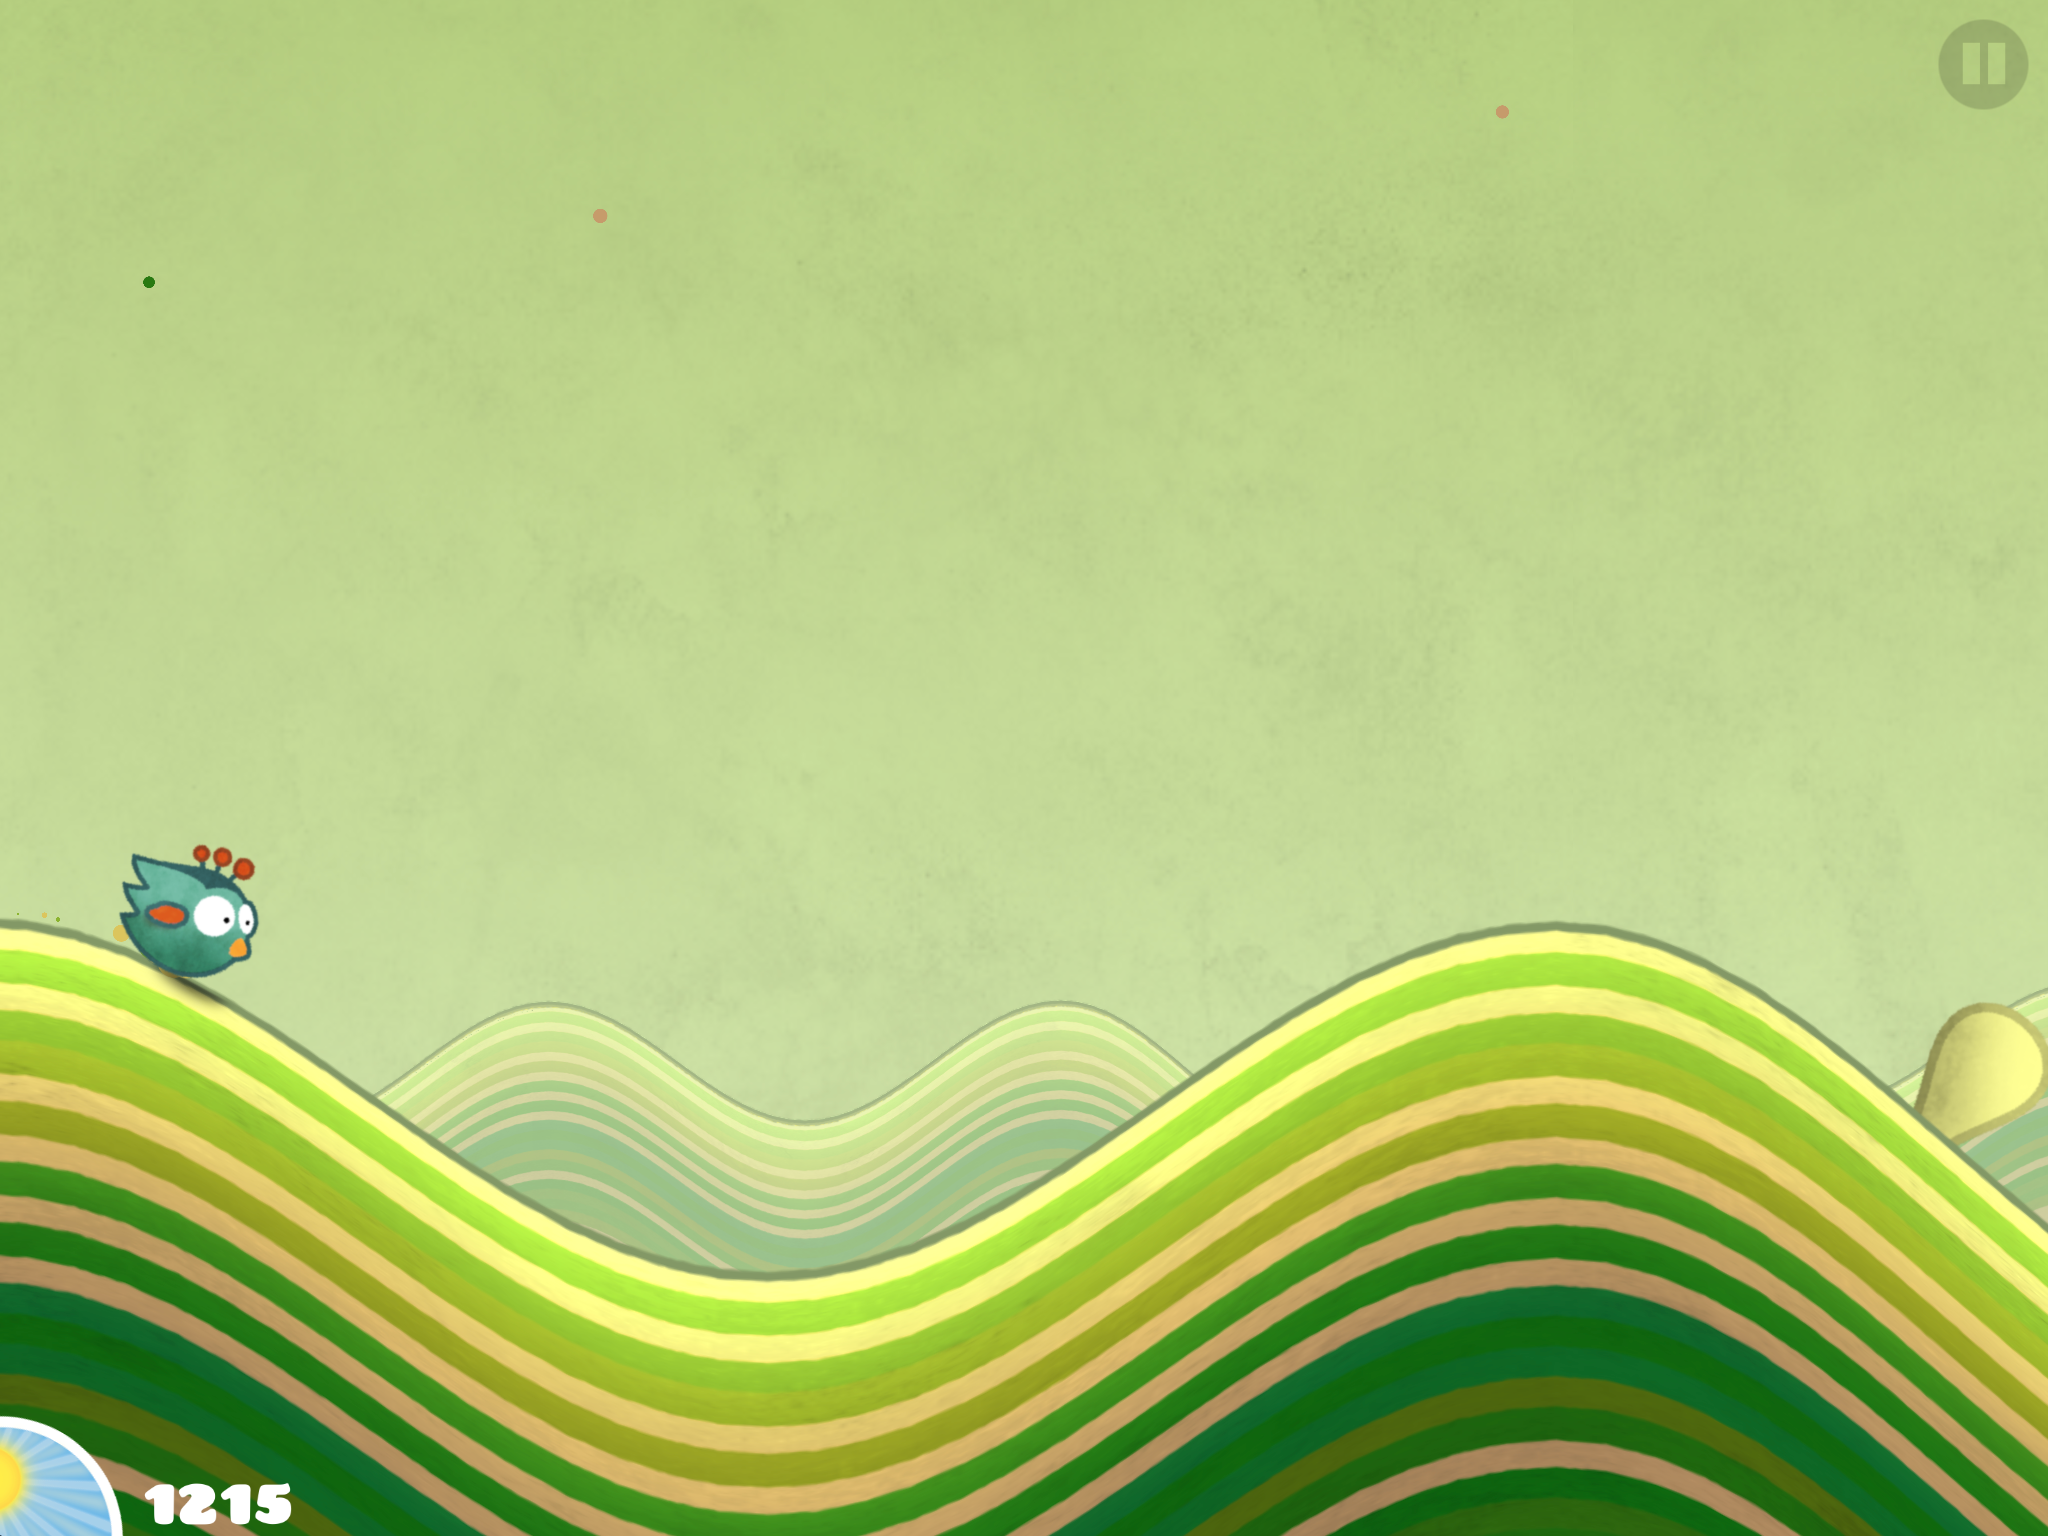
\includegraphics[width=\textwidth,height=0.62\textheight,keepaspectratio]{figures/fig01.png}
\end{center}

我从事理论研究与算法开发工作也恰恰像是翻越一座座连绵起伏的山脉。每一次登顶后，都能收获不尽的欣喜（ecstasy）与鼓舞（encouragement）。然而，这种如释重负（relieving）的感觉往往是转瞬即逝（ephemeral）的，因为眼前会立刻浮现出（loom up）更加高大、巍峨的山峰以待我去征服。此时，我不得不让兴奋的头脑冷静下来，重置在刚刚达成目标、收获成功后的“轻浮”心态，重新聚集力量（strength）、耐心（patience）、专注（focus）、细心（meticulosity），仿佛一切又从零开始一样。

“不忘初心”的口号容易让人获得一种虚无的信心与空洞的自豪。但当它对应到具体的实践与真实的生命体验时，就会以上述清零、重置、重启的感觉呈现，这已近乎无助的努力与绝望的抗战。然而，只有身处于这种体验与状态时，我才会觉得一切都是合理的、正确的、正常的（Alles in Ordnung）。因为这才是开发者的真实状态，也是事物从无到有、不断提升的一般规律，更是有志于学者求仁得仁的命运。

\begin{classic}
《论语·述而篇第七 7.15》冉有曰：「夫子为卫君乎？」子贡曰：「诺，吾将问之。」入曰：「伯夷、叔齐何人也？」曰：「古之贤人也。」曰：「怨乎？」曰：「求仁而得仁，又何怨？」出曰：「夫子不为也。」
\end{classic}

\entrydate{2023.06.15}

\chapter{从心所欲不逾矩}

我在学习与研究的过程中越来越频繁地发现，无论是记笔记、数学推导、代码编写，还是撰写报告与文章，都不再是一蹴而就的，而演变为一个多次迭代、逐步完善的过程。与此同时，在这个过程背后必有一个大致的目标——其实，该目标倒也不一定非常清晰明确，因为我往往都是在黑暗中前行，在未知或者一知半解中摸索的——和一些基本思想、设计原则，以及一贯的做事风格与工作态度等非智力的、无法量化的要素作为冥冥之中的引导。这种模式与我在学生时代的压力与忙碌中为了完成作业、应对考试、准备毕业论文的学习与研究方式是完全不同的。它要求我必须扫除内心所有的浮躁与急迫，以一种不得不依照通过长期持续的科学探索直至有所心得、有所发现需遵循的一般规律来做事。其间绝不能有逻辑上的跳跃与模糊不清，亦容不得弯道超车与自吹浮夸，只能以无比坚实的耐心与细心来推进工作。

一开始，我按这样的方式做事可以说是出于无耐，因为只要有丝毫的马虎大意，出错就总是必然的——这一点我从每次修改程序后第一次编译很容易出错这一现象就可以看出。后来，慢慢地变成了一种“逆来顺受”，且直到今天依然如此。最终，我想应该努力达到从心所欲不逾矩的境界。

\begin{classic}
《论语·为政篇第二 2.4》子曰：「吾十有五而志于学，三十而立，四十而不惑，五十而知天命，六十而耳顺，七十而从心所欲，不逾矩。」
\end{classic}

\entrydate{2024.10.01}

\chapter{命运的最好安排}

算法开发与测试是一项需要高度专注、细致、耐心的工作。因此，动手干活前就不能急躁、毛糙，要将目标和步骤都想清楚后再逐个落实。当然，由于需要处理与消化的信息量较大，且随着个人年龄增长可能出现的记忆力衰退问题，大脑就会记不住那么多信息。此时，可利用白板、思维导图、KNote、Xournal++ 等软硬件工具，将步骤与要点列清楚，将想法用最自由与直接的方式予以表达和记录。不要因为怕麻烦或者不愿切换工作环境与条件而不去启用这些工具。它们就相当于我们无限大的稿纸、记忆力的延伸、工作内存的拓展、想象力的激励。没有这些工具的辅助，仅依赖自己的心算、空想和机械式地推演，是无法将信息内化为理解，也解决不了复杂与深奥的问题的。

上述专注、细致、耐心的工作态度恰与我自己中小学逐渐培养起来的学习态度是一致的。回想起来，在以前的学生时代，我将课本、笔记、习题集、考卷反复揣摩、提炼、重构了无数遍。在每一次的考场上，我虽然在考试结束前很早就已完成了答卷和检查，但仍旧能够 \textbf{不厌其烦} 地在稿纸上多次演算、验证，以确保解题步骤、措词行文、最终答案万无一失、完美无缺。这个过程其实是非常枯燥与乏味的，与我如今在算法开发过程中百思不得其解地调试程序极为类似。而以往通过不断磨炼形成的习惯与风格，正好恰如其分地用在了当前数值算法开发这种精细、精密的工作中，使我获益匪浅。

由之前的因，逐渐形成今日的果。能够让多年以前的素质、态度、模式在当前和未来持续发挥关键性的作用，这便是命运的最好安排！想来，这也是孔子所说的“吾道一以贯之”在科学研究上的具体体现。

\begin{classic}
《论语·里仁篇第四 4.15》子曰：「参乎！吾道一以贯之。」曾子曰：「唯。」子出。门人问曰：「何谓也？」曾子曰：「夫子之道，忠恕而已矣。」

《论语·尧曰篇第二十 20.3》子曰：「不知命，无以为君子也。不知礼，无以立也。不知言，无以知人也。」
\end{classic}

\entrydate{2024.01.30}

\chapter{无友不如己者}

虽然我并不是顶级聪明的人，但是在实践中发现，通过长时间地思考和玩味一个问题，确实能够使自己的认知获得质的提升。这个提升的达成是随机出现的。你可以把这个现象归因为灵感和运气。虽然看似飘忽不定、不可捉摸，但其产生是有必然性的。因此，在长期保持专注的前提下，对于顿悟与灵光一现要抱以十足的信心。这是对于勤能补拙这个道理在实践上的验证，而不仅仅是在理性与情感上的形式认可。所以说，王阳明“知行合一”的说法是绝对正确的，只有通过笃行才能够获得对人生、做事等各方面道理的真正理解。

耐心、细致、扎实地工作，不要着急。既要自由涂鸦、大胆改动、发散思考，又要耐心、谨慎地推理，不断调用和累积细致入微的知识点。要通过反复的训练、反省、改进，将这两种工作模式很好地融合起来，做到从心所欲不逾矩。虽然开发区域分解算法涉及的细节和步骤非常多，而且他们在脑海里的浮现也是有一定的随机性，越是这种看似的紊乱，越要耐下性子，一点一点地做，一点一点地想和记录，最终一定能够从纷繁芜杂中逐步走出来。

面对这种复杂的开发工作，也越来越深刻地体会到工具的重要性。譬如机械加工，高精度的零件只有借助精密的机器、精湛的技艺、合理的加工流程才能做出来。同样的，无论是理论推导、软件设计、算法开发，还是记笔记与信息管理，工具的功能是否足够强大，你对它是否投入了足够的时间以便操作熟练并且持续扩展其功能、提高效率，在很大程度上决定了你能够做成事情的复杂度、精密度和质量。所以，任何时候都不要投机取巧，都不要为了图快而采用退而求其次的方案。所以，将正则表达式、软件项目构建与调试工具、二进制文件的操作命令等基本工具用对、用熟、用好，才能完整地实现自己的设计思想。否则，就只能是处处妥协，处处打折扣，浮沙筑台，最终根本构建不起大的项目。

当下碎片化信息多以短视频形式传播。长篇表达如会议演讲、系统化信息讲授如大学课程也多以视频形式发布。然而，话虽说得好，道理讲得通透，经过了前期设计与后期制作，表达形式也变得生动光鲜，但大多容易陷入巧言令色、论笃行浅的境地。对此，我们要予以明辩：究竟主讲者是真君子、真学者，还是仅仅表现得人模人样，只有言语技巧或者文字功夫。一个评判的标准是，不要看这个人说了什么、领导或组织了什么，而要看这个人亲力亲为做了什么，实践过程是否贯彻了其所讲的思想与原则，收获的成果是否也体现了同样的品质精神。

\begin{classic}
《论语·先进篇第十一 11.21》 子曰：「论笃是与，君子者乎？色庄者乎？」
\end{classic}

因此，我们根本不必知道那些不如自己或跟自己差不多水平的人所做的工作以及采用的态度、方式。要和这个世界上最优秀的、亲力亲为的人对比、参照，以他们为榜样，如 Linus Torvalds，Richard Stallman。想要有真正的创新，想要做出能够打动人心的工作，首先就不能对现实妥协，要敏锐且不留情面地发现其中的问题，不断改进。若只是被动地适应周遭的环境，成为与中低水平同类内卷过程中的赢家，最终看似收获颇丰，但那只不过是病态的毒瘤，越多反而越糟。千万不要以为大的、多的就是好的。真正的优雅和顶级的品质与数量和规模无关。

\entrydate{2024.08.23}

\chapter{如何面对“无底洞任务”}

我们在生活中总会遇到一些工作量大到几乎是无穷或者难以估计的任务，如数学学习与研究这类既重要又紧急的工作。它们堪称消耗个人时间和精力的无底洞。而如何将其与生活中的其他事务平衡与协调起来，就成为一个颇为困扰的问题。毕竟，个人学识的长进与修养的提升是无法仅凭藉在单一或极少数几个领域中的专注就能够达成的。这是因为不同领域在思想方法和“悟道”的层次上都是相通的。例如，通过音乐、体育的训练总结出的有效方法、宝贵经验，甚至仅仅是一些流动的心理感受，就可以触类旁通、移花接木般地从中收获对纯粹理性工作的启发。此外，生活中亦还有其他非常重要的事情需要精心打理，如家庭、亲情、友情的经营与维护。然而，“无底洞任务”的存在势必会在时间、精力、心理上对其他任务产生强大的挤压作用，令人极难作出决策与取舍。

对此，我觉得如果能够把握以下三个原则，将会有助于上述困境的解决。

\begin{itemize}
\item 要构建并固化属于个人的学识发展框架。这相当于站在完整人生的战略高度，在整体架构和门类上对个人的学习、研究、工作、爱好的范畴予以界定。而“无底洞任务”无疑就是这个框架的基石或核心。这也就是儒家思想中的“止于至善”、“君子务本，本立而道生”。立于这个坚如磐石的基础上，一个人才会对“无底洞任务”的规划与执行产生信仰般的持久动力。否则，无论外在环境或者他人的观点意见有任何惊涛骇浪或细小波澜般的变动，你的心态和行动都会受到影响和干扰，此即“小人之德草，草上之风必偃”。
\item “罗马不是一天建成的”。即便是焚膏继晷、不饮不食，也不可能在短时间内搞定“无底洞任务”。所以，还是放弃这种不切实际的念想吧！相反，要将其当作长期的追求。不过，需要留意的是，万万不可把长期的追求抽象地扩展为“毕生”的追求。那样一来，就没有了紧迫感，无法形成自我压力。稍有不慎，就变成了踩着西瓜皮行走，得过且过了。因此，需要制定带有截止日期的中长期计划。关于计划的作用可以参考罗辑思维第236期《计划的用处》。其中提到了计划并不是为了死板和教条地照章办事，而是给自己创造出一个可以基于理性思考的判断、评估和决策的机会。同时，计划亦是在团队中达成共识、形成凝聚力的必要因素。至于现实中会出现什么样的变化，则可以根据具体情况予以更改。
\item 将“无底洞任务”拆解为可以执行的步骤。只有做到对于细节任务的明晰与把控，才不至于在宏观问题上产生迷茫甚至动摇。若你觉得“无底洞任务”令人畏惧，深不可测，那就证明你对于如何开展和实施它们思考得不够多、不够细，以至于拿不出一个成文的任务清单。而一个经过理性思考后得出的任务清单即便不甚合理，也总比什么都没有强。更何况，任务分解的合理性也并不是一个可以先验地予以回答的问题。相反地，只有通过具体的执行逐渐获取更多的信息，并时时反思、修正，才可以逐渐地逼近真值。可以看出，“敏捷开发”的思想方法也在此得到了应用。在任务分解的过程中需要秉持的心态是：“磨刀不误砍柴工”，宁可慢，不宜快。虽然从最初的分析、思考再到最终的成形需要花费很多时间，但是这样的投入能够保障人生航向的正确或者是自以为正确，从而获得强大的自信与自我说服力，因而是极其值得的。
\end{itemize}

总之，如果你的生活中存在“无底洞任务”，虽然表面上看似可怕，但也未尝不是一件好事：因为这至少证明了在你的生命中还存在值得长期坚持的元素，它们的价值和意义远远超出了每天朝九晚五的工作和柴米油盐的生活。然而，为了把“无底洞任务”和自己的生活协调好，就需要信仰般地确立属于自己的学识架构，在宏观上为其制定出带有截止日期的中长期计划，在微观上拆解出可以照章办事的任务列表。同时需要注意的是，计划的存在绝不意味着教条与死板，而是意味着理性思考和对不断变化环境的自适应。

\begin{classic}
《论语·学而篇第一 1.2》 有子曰：「其为人也孝弟，而好犯上者，鲜矣；不好犯上，而好作乱者，未之有也。君子务本，本立而道生。孝弟也者，其为仁之本与！」

《论语·颜渊篇第十二 12.19》 季康子问政于孔子曰：「如杀无道，以就有道，何如？」孔子对曰：「子为政，焉用杀？子欲善，而民善矣！君子之德风，小人之德草，草上之风必偃。」

《论语·子路篇第十三 13.17》 子夏为莒父宰问政。子曰：「无欲速，无见小利。欲速则不达，见小利则大事不成。」
\end{classic}

\entrydate{2017.11.26}

\chapter{数学与长笛}

数学理论的大厦乍一看上去令人瞠目结舌：其规模的宏大伟岸，外延的似无边际，内涵的深不可测，抽象分类的层出不穷，逻辑联结的精密繁杂，以及千变万化的诸多变换，令人深感自身渺小，不由心生敬畏甚至恐惧。然而，若将其拆解为一个个细小但彼此相连的定义、定理，我们就还是可以如同蚂蚁啃骨头一般，把它们逐渐理解、消化乃至最终掌握的。

与数学类似，长笛演奏同样是一门博大精深的学问，而且还包含了很多难以言表、只能先经老师点拨再靠自己体悟的技能、艺术。尽管如此，也还是可以在练习的过程中将其拆解为不同的方面，如基本功、练习曲、表演曲、乐理。其中，基本功又可以分解为长音、颤音、双吐音、强弱变换、基于音阶的快速指法等。而练习曲和表演曲则可划分为很小的乐句乃至每一个小节，然后精雕细琢、精益求精地去练习。这包括对于指法的感受和熟悉，呼吸与情绪的把控，强弱、快慢和节奏的处理，音色与表现力的微调等等。乐理知识则是一门独立的学问，需要以研究的心态来吸收、揣摩。

由以上可以看出，数学学习和长笛练习是相通的。她们无一不是要经过仔细考虑、反复斟酌、不断强化练习和“如临深渊”般的精准控制。毕竟，要想臻于完美，就需要在修炼和磨练的过程中克服畏难情绪，拥有无与伦比的耐心，付出大量的苦心和苦功。

\begin{classic}
《论语 子罕 9.15》子曰：“吾自卫反鲁，然后乐正，雅颂各得其所。”

《诗经 小雅 小旻》战战兢兢，如临深渊，如履薄冰。

《论语·泰伯篇第八 8.3》 曾子有疾，召门弟子曰：「启予足！启予手！诗云：『战战兢兢，如临深渊，如履薄冰。』而今而后，吾知免夫！小子！」

《论语·学而篇第一 1.15》 子贡曰：「贫而无谄，富而无骄，何如？」子曰：「可也，未若贫而乐，富而好礼者也。」子贡曰：「诗云：『如切如磋，如琢如磨』，其斯之谓与？」子曰：「赐也，始可与言诗已矣，告诸往而知来者。」

《论语·八佾篇第三 3.23》 子语鲁大师乐，曰：「乐其可知也：始作，翕如也；从之，纯如也，皦如也，绎如也，以成。」
\end{classic}

\entrydate{2017.10.26}

\chapter{学习与研究自由}

自学数学最好能配有一本与个人拥有的理论基础和知识体系、对学科背景和发展历史的了解程度、习惯的逻辑推演和表述方式相契合，且推导过程细致入微、鲜有逻辑跳跃，同时又能上升到方法论层次而授人以渔的优秀教科书或专著。单就内容组织与数学推导的细致程度来说，当以德国人的著作更胜一筹（Teutonic thoroughness）。正所谓凡事怕认真二字，而“细致”便是“认真”的一个重要而具体的体现。

若想在我们的研究历程中与这类著作邂逅并产生交集与共鸣，首先需要自身的刻苦努力。毕竟，只有通过广泛阅读与一定深度的学习，才能对涉及同一领域、同一研究问题的不同著作有所切身感受和对比，由此才能作出选择。网上的书评与书单只代表了他人的感受与意见，因而仅能作为我们文献调研的参考与起点，而绝不能替代我们自身的实践、体验与评判。其次，能够遇到适合自己的书籍也需要某种难以捉摸和把控的缘分。不过在当今信息资源丰富、搜索工具强大便利的条件下，能够找到属于自己并引领我们进入更宏伟理论殿堂的书也变得相对容易些了。

上述调研、阅读、评判的过程，恰是促进我们实现 \textbf{学习与研究自由} 的重要一步。而这个自由远胜过财富自由。毕竟，变富虽能让一个人用财富杠杆轻松撬动“现实”成果，但也容易使其计较过多、乐不思蜀，从而成为在“求真”层面上自我提升的障碍，并终究难以重返宁静、深思冥想、付出苦功、下学上达。

\begin{classic}
《论语·宪问篇第十四 14.35》 子曰：「莫我知也夫！」子贡曰：「何为其莫知子也？」子曰：「不怨天，不尤人，下学而上达。知我者，其天乎！」

《论语·学而篇第一 1.15》 子贡曰：「贫而无谄，富而无骄，何如？」子曰：「可也，未若贫而乐，富而好礼者也。」子贡曰：「诗云：『如切如磋，如琢如磨』，其斯之谓与？」子曰：「赐也，始可与言诗已矣，告诸往而知来者。」
\end{classic}

\entrydate{2022.07.03}

\chapter{三人行，必有我师焉}

现在回想起来，自己曾在大学从本科到博士后度过了整整十一年的荏苒时光，而屈指算来人生也就不过八到十个十年而已。原以为自己的人设就是在学校终老一生、与学术为伴的，但最后也从中跳出来到了外企工作，至今竟也整整七年了。虽说学校是学生们得以专注学习、潜心研究的象牙塔，是慎思博学的风水宝地，但一个人到了工作中、社会上，只要凡事处处留心，待人虚怀若谷，也仍有不少甚至是学校都难以或无法提供的学问与心法。本文便将我工作数年期间从学长、同事那里学到的思想方法与相关的个人心得体会整理罗列出来，旨在通过回顾与重温来加深印象，从而既有助于自修，也提醒自己不忘感恩，此外若还能对更多的人有所启发与裨益，则更是值得欣慰了。

\begin{itemize}
\item 搜索与阅读专著和文献时，需要带着明确目标去查阅真正对解决问题有用的材料。要有细节但又不能拘泥于细节。要能够分清不同任务的轻重缓急，明确什么是自己最擅长的，什么又是自己需要去发展的。这应该就是做科研的艺术！由此，才可以确定应该在哪些事上做得更底层一些，而在哪些事情上又需要大胆地站在前人的肩膀上，利用他们已有的成果。
\item 眼高手低是做技术者的大忌，尤其是自以为智商过人的时候。即便是对于已经掌握较好的技术，也不能因骄傲和自满而停滞不前，应该持续学习、不断提升，达到行云流水的境界。
\item 无论是纯粹理论的推导还是工程技术方案的实现，都像是俄罗斯套娃一样层层相套、相扣。只有不厌其烦，逐层地打开这些黑盒子，尽可能展开更多的细节，才能够暴露更多潜在的问题。也只有如此，才能够获得大量数据用以澄清问题，并将其逐一解决，从而最终保证整个技术实现的完全精确与可靠。
\item 止于至善的精神不仅仅适用于长期的、终极的人生，也完全适用于项目工作的开展。至善，就像是油画中的所有细节那样，是不知经过多少次细枝末节的修改、增删而一层一层地积累起来的。想要止于至善，就必须培养起足够的乃至惊人的耐心与毅力。不怕慢，不怕细，不怕反复，更不怕屡次的失败与推倒重来！
\item 面对不直接参予技术实施的项目负责人以及对技术只知皮毛概念的高层管理者，要想阐释什么是正确的、证明什么才是真理的最好方法不是用数学和物理理论，而是实验数据和技术演示。因为到了职场中、社会上，已经鲜有人有能力和耐心去跟你一起做逻辑推演了。
\item 要想让项目提议获得管理层的认可，并在其实际支持下从幼苗成长为大树，需要编制与展示完整的用户故事，而不是灵光一现的理论方法、前沿技术，即便该理论与技术是项目的核心与精髓。毕竟，对于管理层与最终用户来说，直接创造价值的是产品不是技术。从另一方面讲，被人认可的只是产品的实用价值而无人关心和欣赏背后的设计，这也是科技工作者的悲哀。正所谓，“欲将心事付瑶琴，知音少，弦断有谁听？”。
\item 对于技术可行性一定要有明确的表态，尤其是能否做成的表态。否则，会让别人做出错误的决策，以至于本来还有其他挽救的方案但却没有采用。
\item 进入职场的时间长了，人就容易疲，容易自满与浮躁。此时，要将自我清零，像小学生面对老师一样，怀着一颗无比耐心与踏实的心。
\item {\kaishu 《大学》中说到的“正心诚意”，不仅指对待自己的本职工作，在给同事提供力所能及的协助时也应同样如此。这便是“尽己”与“不辱使命”。}
\end{itemize}

\begin{classic}
《论语·述而篇第七7.22》 子曰：「三人行，必有我师焉：择其善者而从之，其不善者而改之。」
\end{classic}

\entrydate{2018.10.27}

\chapter{文献阅读方法改进}

在学术文章与专著的阅读方面，我发现自己稍不留神便常常走入如下两个极端：

\begin{itemize}
\item 过尤不及：过于认真地阅读以至进度极其缓慢。虽然也吸收了相当多的细节内容，但却对原本的学习目标贡献寥寥。这种情况便是事倍功半。（《论语·先进篇第十一11.16》 子贡问：「师与商也孰贤？」子曰：「师也过，商也不及。」曰：「然则师愈与？」子曰：「过犹不及。」）
\item 走马观花：一味追求效率和进度，以跳跃和不求甚解的模式浏览原文。结果看了一圈下来，不晓得主旨，抓不住要领，白白浪费了时间和精力。这时，所谓的效率其实已经“堕落”成浮躁，实质性的进度则为零。（《论语·子路篇第十三13.17》 子夏为莒父宰问政。子曰：「无欲速，无见小利。欲速则不达，见小利则大事不成。」）
\end{itemize}

由此可以看出，在认真细致与高效粗略之间，我还拿捏不好分寸。需要进一步通过提高阅读量、记录和整理出的笔记量（关于笔记量，在《The Man Who Knew Infinity》一书中讲到拉马努金（Ramanujan）每月都要写两千多页（He'd need four reams of it a month.）的数学推导和演算草稿。与在如此专注和勤奋的状态下产出的工作量相比，我还有相当大的差距。），以及复习的频率，以期得到改进。具体的整改措施罗列如下：

\begin{itemize}
\item 在开始阅读前，明确自己的阅读目标（target）、期望的收获（deliverable）和预计投入的阅读时间（resource）。在训练初期，由于对阅读技巧的把控尚未做到游刃有余，需将这三方面内容逐条清晰且尽可能量化地列在清单中。然后，便可以该清单作为阅读过程中的即时提醒和阅读完成后的考核标准。注：这里所谓的即时提醒，起到的是“君子无终食之间违仁”的效果。（《论语·里仁篇第四 \quad 4.5》子曰：「富与贵，是人之所欲也，不以其道得之，不处也。贫与贱，是人之恶也，不以其道得之，不去也。君子去仁，恶乎成名。君子无终食之间违仁，造次必于是，颠沛必于是。」）
\item 在需要认真细读的地方，应以期望的收获作为指引，把每一个环节都想得如水晶般透彻，并工整地做好笔记。笔记的整洁与否，以及是否具有形式上的结构化、内容上的条理性和最终体系的完整性，能够反映出一个人的心态是平静还是躁动，思路是清晰还是紊乱，思想是深刻还是浮浅。因此，不可不引起高度重视。
\item 在需要高效略读的地方，要围绕自己的阅读目标，紧紧抓住文章或书籍的主旨思想、重要方法、技术环节、主要结论等几个关键要素，从而展开快速的阅读活动。不应一味徒快，以至于花费了时间与精力，但脑海仍旧空空如也。
\end{itemize}

\begin{classic}
《论语·先进篇第十一 11.16》 子贡问：「师与商也孰贤？」子曰：「师也过，商也不及。」曰：「然则师愈与？」子曰：「过犹不及。」

《论语·子路篇第十三 13.17》 子夏为莒父宰问政。子曰：「无欲速，无见小利。欲速则不达，见小利则大事不成。」

《论语·里仁篇第四 4.5》 子曰：「富与贵，是人之所欲也，不以其道得之，不处也。贫与贱，是人之恶也，不以其道得之，不去也。君子去仁，恶乎成名。君子无终食之间违仁，造次必于是，颠沛必于是。」
\end{classic}

\entrydate{2018.10.09}

\chapter{避免对工具的痴迷}

工具作为拓展人类智力与能力的利器，其自身所具备的功能、性能、可扩展性的重要意义毋庸置疑。一个人也应当持续不断地通过刻意练习来提升使用工具的能力，达到熟能生巧、能够自然流畅地表达设计思想与技术理念的效果。但与此同时，亦不要对某种技术或者软件工具怀有太多的感情与痴迷，更不要卷入诸如网上Vimer与Emacser之间的论战与纷争。这主要是出于下面的考虑。

一个工具的流行程度会随着时代的变迁与技术的演进而不断变化，甚至完全被淘汰。举例来说，曾经红极一时的Perl语言如今逐渐淡出人们的视野，而昔日因性能太慢而被大家鄙视吐槽的Python反倒成了当下大红大紫的名星。因此，优秀的科技工作者应该关注隐身于工具与技术背后那些真正稳定甚至是永恒的要素：设计思想（包括数据与算法的抽象、软件的组织架构等）以及需要解决的具体问题（“解决问题”、“改善生活”是人类得以延续和发展的持续动力）。然后，在此基础上更进一步，通过数学【理论】与泛型编程【实践】的高度抽象来解决一大类问题而非单个案例。相反地，不能仅仅因为已经在一个技术上投入了大量学习与实践的时间并拥有了相当多经验与技能的积累，便始终持有一份情怀与坚持不放。这样一来，身上背负的“历史”包袱只会越来越重，最终则被时代无情地抛弃。总之，大多数的技术需要深厚的积累方能形成强大的生产力与推动力，但却不能固守。开发者仅将它们当作称手的工具解决当下的问题，不需要的时候扔掉即可，与时俱进。

换个角度来看，最终用户关心的则是由工具创造出的产品而绝非工具本身。除了开发者自己对于工具有着一份执念与情怀外，用户是丝毫不会关心工具本身有多么强大和先进的。开发者能够与用户建立起的唯一接口就是产品能够达到的性能、实现的效益和形成的体验。因此，理性的开发者应当更多地关注用户的需求与体验，通过整合现有的知识与工具勾画出完整的“用户故事”，精益求精地实现与之相应的解决方案。这也是《论语》所说的“吾日三省吾身，为人谋而不忠乎？”。

\begin{classic}
《论语·学而篇第一 1.4》 曾子曰：「吾日三省吾身，为人谋而不忠乎？与朋友交而不信乎？传不习乎？」
\end{classic}

\entrydate{2020.06.13}

\chapter{“学之不讲”是吾忧也}

\begin{classic}
《论语·子罕篇第九 9.29》子曰：「知者不惑，仁者不忧，勇者不惧。」

《论语·述而篇第七 7.3》子曰：「德之不修，学之不讲，闻义不能徒，不善不能改，是吾忧也。」
\end{classic}

“学之不讲，是吾忧也”，这句话恰如其分地描述了我现在的心情：面对积累的越来越多的知识，我对它们并非全都有过具体、反复的操练，所以根基并不扎实，前学后忘便很难避免。在做事、实践的过程中，我总会感到“书到用时方恨少”。但与此同时，又不能陷入复习、练习的无限循环中，而始终不能从中跳出来做事、实践。单独来看学习、复习、练习、实践，每一项似乎都还可以应对（当然，否能够做得好就另当别论了）。但将这四者放在一起，且考虑随时间积累的倍增因素，就会发现时间根本不够用，人生的紧迫感也就由此而生。

这也就是为什么虽然孔子曾说过“仁者不忧”，但具体到做学问乃至修德、行善的时候，面对人生“不舍昼夜”的紧迫感，忧虑就不可避免了。然而，只是忧虑是不行的，还要将其化解，将压力转变为动力，再以放松的身心投入到做学问中，这样才能获得最好的效果。在这一点上，孔子的做法则是直接或者间接地（通过文学作品）走入与感悟大自然，即 living in communion with nature。例如，

\begin{classic}
《论语·先进篇第十一 11.26》「莫春者，春服既成；冠者五六人，童子六七人，浴乎沂，风乎舞雩，咏而归。」夫子喟然叹曰：「吾与点也！」

《论语·雍也篇第六 6.23》子曰：「知者乐水，仁者乐山。知者动，仁者静。知者乐，仁者寿。」

《论语·阳货篇第十七 17.9》子曰：「小子！何莫学夫诗？诗，可以兴，可以观，可以群，可以怨。迩之事父，远之事君，多识于鸟兽草木之名。」

《论语·子罕篇第九 9.28》子曰：「岁寒，然后知松柏之后雕也。」

《论语·子罕篇第九 9.17》子在川上曰：「逝者如斯夫！不舍昼夜。」

《论语·乡党篇第十 10.27》色斯举矣，翔而后集。曰：「山梁雌雉，时哉时哉！」子路共之，三嗅而作。
\end{classic}

同时，聆听音乐也是对心灵最好的净化与抚慰。

\begin{classic}
《论语·八佾篇第三 3.23》子语鲁大师乐，曰：「乐其可知也：始作，翕如也；从之，纯如也，皦如也，绎如也，以成。」

《论语·述而篇第七 7.14》子在齐闻韶，三月不知肉味，曰：「不图为乐之至于斯也。」

《论语·泰伯篇第八 8.8》子曰：「兴于诗，立于礼，成于乐。」

《论语·子罕篇第九 9.15》子曰：「吾自卫反鲁，然后乐正，雅颂，各得其所。」
\end{classic}

两千多年过去了，以上这些语录依旧能给我们带来心智的启发与实践的指导，想来真的是很神奇。相较于科技发展的日新月异，人性真的是蛮稳定的。

\entrydate{2024.05.02}
